\include{settings}

\begin{document}	% начало документа

% Титульная страница
\begin{titlepage}	% начало титульной страницы

	\begin{center}		% выравнивание по центру

		\large Санкт-Петербургский политехнический университет Петра Великого\\
		\large Физико-механический институт \\
		\large Высшая школа прикладной математики и вычислительной физики\\[3cm]
		% название института, затем отступ 6см
		\large Направление подготовки\\
		\large "01.03.02. Прикладная математика и информатика"\\[3cm]
		\huge Дисциплина "Численные методы"\\[0.5cm] % название работы, затем отступ 0,5см
		\large Отчет по лабораторной работе №4\\[0.1cm]
		\large "Решение алгебраической проблемы собственных значений итерационными методами. Степенной метод для поиска второго максимального по модулю собственного значения и соответствующего собственного вектора"\\[5cm]

	\end{center}


	\begin{flushright} % выравнивание по правому краю
		\begin{minipage}{0.25\textwidth} % врезка в половину ширины текста
			\begin{flushleft} % выровнять её содержимое по левому краю

				\large\textbf{Работу выполнил:}\\
				\large Иванова А.С.\\
				\large {Группа:} 5030102/00002\\
				
				\large \textbf{Преподаватель:}\\
				\large Курц В.В.

			\end{flushleft}
		\end{minipage}
	\end{flushright}
	
	\vfill % заполнить всё доступное ниже пространство

	\begin{center}
	\large Санкт-Петербург\\
	\large \the\year % вывести дату
	\end{center} % закончить выравнивание по центру

\end{titlepage} % конец титульной страницы

\vfill % заполнить всё доступное ниже пространство


\include{ToC}

\section{Формулировка задачи}

Дана матрица 
\begin{math}
	A\in R^{nxn}
\end{math}
с собственными числами, упорядоченными по модулю. Найти второе максимальное по модулю собственное число и соответствующий собственный вектор, используя модификацию степенного метода.

Исследовать сходимость (число итераций от 
заданной точности) при хорошей и плохой отделимости искомого собственного числа. 

\section{Алгоритм метода и условия его применимости}

\subsection {Условия применимости}

Матрица А должны быть матрицей простой структуры

\subsection {Алгоритм метода}

\begin{math}
	A=A^{T} => (w^{(i)},w^{(j)})=\delta_{ij} 
\end{math}
где 
\begin{math}
	w^{(i)} 
\end{math}
- собственные векторы А

Пусть максимальное по модулю собственное число
\begin{math}
	\lambda_{1} 
\end{math} и соответствующий собственный вектор
\begin{math}
	w^{(1)} 
\end{math} уже найдены.

Возьмем произвольный вектор 
\begin{math}
	x^{(0)} \in R^{n}
\end{math}
n и разложим его по ортонормированному
базису из собственных векторов. 

\begin{math}
	x^{(0)}=\sum_{j=1}^{n}\alpha_{j}w^{(j)}
\end{math}

\begin{math}
  y^{(0)}= x^{(0)}-\gamma w^{(1)}
\end{math}
выберем так, чтобы
\begin{math}
   (y^{(0)},w^{(1)})=0 => \gamma=\alpha_{1} => 
\end{math}

\begin{math}
	y^{(0)}=\sum_{j=2}^{n}\alpha_{j}w^{(j)}
\end{math}

Пусть соственные числа упорядчены по модулю.

Можно применять степенной метод 

\begin{math}
	y^{(k)}=A^{k}y^{(0)}=\alpha_{2}\lambda_{2}w^{(2)} (1+O(|\frac{\lambda_{3}}{\lambda_{2}}|^{k}))
\end{math}

Если проводить ортогонализацию на каждом шаге, то итерационная послеовательность строится по формулам 

\begin{math}
  x^{(k)}=Ay^{(k-1)}
\end{math}

\begin{math}
	y^{(k)}=x^{(k)}-\gamma w^{(1)}
\end{math}

Критерий для остановки итерационного процесса. Пусть 
\begin{math}
	\lambda^{*}
\end{math}
и
\begin{math}
	x^{*}
\end{math}
- приближенное собственное значение и приближенный собственный вектор соответственно.

Тогда 

\begin{math}
	\epsilon=|\lambda_{A}-\lambda^{*}|<=\frac{||Ax^{*}-\lambda^{*}x^{*}||_{2}}{||x^{*}||_{2}}
\end{math}

\section{Предварительный анализ задачи}

Для того, чтобы метод сходился, необходимо, чтобы матрица А являлась матрицей простой структуры. Следовательно с помощью преобразований ее можно привести к диагональному виду. 

\begin{math}
	G^{-1}AG=diag{\lambda_{i}}
\end{math}

Будем строить матрицы следующим образом: 

\begin{math}
	D=diag{\lambda_{i}}
\end{math}

Генерируем ортогональную матрицу Q и получаем матрицу А:

\begin{math}
	A=Q^{-1}DQ
\end{math}

Таким образом мы получаем матрицу простой структуры, следовательно условие выполнено.

\section{Проверка условий применимости метода}

Для того, чтобы метод сходился, необходимо, чтобы матрица А являлась матрицей простой структуры. Следовательно с помощью преобразований ее можно привести к диагональному виду. 

\begin{math}
	G^{-1}AG=diag{\lambda_{i}}
\end{math}

Будем строить матрицы следующим образом: 

\begin{math}
	D=diag{\lambda_{i}}
\end{math}

Генерируем ортогональную матрицу Q и получаем матрицу А:

\begin{math}
	A=Q^{-1}DQ
\end{math}

Таким образом мы получаем матрицу простой структуры, следовательно условие выполнено.


\section{Тестовый пример с детальными расчетами для задачи малой размерности}

Дана матрица А:

\begin{equation*}
	A =
	\begin{pmatrix}
		1.6265  & -0.0777 & -0.5017\\
		-0.0777 & 2.7178 & -0.5963\\
		-0.5017 & -0.5963 & 1.6557
	\end{pmatrix}
\end{equation*}

Наглядно видно, что данная матрица является симметричной, следовательно является матрицей простой структуры.

Ее собственные числа приближенно равны 

\begin{math}
 \lambda_{1}=3,\lambda_{2}=2, \lambda_{3}=1
\end{math}
 
 Пусть первое собственное число 
 \begin{math}
 	\lambda_{1}=3
 \end{math} 
первый собственный вектор 
\begin{equation*}
	w^{(1)} =
	\begin{pmatrix}
		 0.0588 \\
		0.4844 \\
		-0.2366
	\end{pmatrix}
\end{equation*}
 уже найдены с помощью обычного степенного метода. 
 
 
 В итоге должно получиться:
 
  \begin{math}
 	\lambda_{2}=2
 \end{math} 
 
Находим нулевое приближение

\begin{math}
	y^{(0)}= x^{(0)}-\gamma w^{(1)}
\end{math}

Для этого находим 
\begin{math}
	\gamma
\end{math}
по формуле: 

\begin{math}
	\gamma=\frac{(x^{(0)},w^{(1)})}{(w^{(1)},w^{(1)})}=1.0424
\end{math}

\begin{equation}
	y^{(0)}= x^{(0)}-\gamma w^{(1)}=
	\begin{pmatrix}
		0.9388 \\
		0.4951 \\
		1.2466
	\end{pmatrix}
\end{equation}

Находим следующее приближение: 

\begin{math}
	x^{(1)}=Ay^{(0)}
\end{math}

\begin{math}
	\gamma=\frac{(x^{(1)},w^{(1)})}{(w^{(1)},w^{(1)})}=1.8876*10^{-16}
\end{math}


\begin{math}
	y^{(1)}= x^{(1)}-\gamma w^{(1)}
\end{math}

Получаем: 

\begin{equation}
	y^{(1)}
	\begin{pmatrix}
		0.8629 \\
		0.5292 \\
		1.2979
	\end{pmatrix}
\end{equation}


\begin{math}
	x^{(2)}=Ay^{(1)}
\end{math}


И так далее: 

Параллельно будем вычислять собственные числа и собственные вектора (v-приближенный сосбтвенный вектор)

\begin{equation}
	x^{(2)}=
	\begin{pmatrix}
		0.7114 \\
		0.5974 \\
		1.4026
	\end{pmatrix}
\end{equation}

\begin{math}
	\lambda_{2}^{(2)}=0.7144/0.8629=0.9193
\end{math}

\begin{equation}
	v^{(2)}=
	\begin{pmatrix}
		0.9388 \\
		0.5756 \\
		1.4118
	\end{pmatrix}
\end{equation}

\begin{equation}
	x^{(3)}=
	\begin{pmatrix}
		0.4082 \\
		0.7340 \\
		1.6050
	\end{pmatrix}
\end{equation}

\begin{math}
	\lambda_{2}^{(3)}=0.8244
\end{math}

\begin{equation}
	v^{(3)}=
	\begin{pmatrix}
		1.0468 \\
		0.8791 \\
		2.0605
	\end{pmatrix}
\end{equation}

Продолжаем итерационный процесс, пока не будет выполнен критерий остановки: 

\begin{math}
	\epsilon=|\lambda_{A}-\lambda^{*}|<=\frac{||Ax^{*}-\lambda^{*}x^{*}||_{2}}{||x^{*}||_{2}}
\end{math}

\section{Перечень контрольных тестов для иллюстрации метода}

Генерируются матрицы размером 10 на 10. Выявляется зависимость количества итераций от точности решения и от отделимости собственных чисел. Ожидается, что чем меньше отделимость, тем большее количество итераций потребуется для нахождения решения с заданной точностью. Точность для нахождения первого максимального СЧ 10е-12, для второго меняется в цикле от 10е-12 до 10е-1

Отделимость для второго собственного числа задается формулой:
\begin{math}
\frac{\lambda_{3}}{\lambda{2}}
\end{math}
Проверяются значения 1/10, 1/5, 9/10, 9.999/10

Матрицы генерируются следующим образом: последние 13 собственных чисел для всех одинаковы, первые два меняются в соответствии с заданной отделимостью.

Наибольшее собственное число и соответствующий собственный вектор ищется с помощью степенного метода с нормировкой.

Также исследуется зависимость количества итераций от отделимости собственных чисел при фиксированной точности 10е-12, отделимость меняется в цикле. Матрицы генерируются таким же образом

\section{Модульная структура программы}

double** ArrayRead(FILE* file, int line, int column)

\includegraphics[scale=0.7]{block1.pdf}

double* Multiplication(double** matrix, double* vector, int size)

\includegraphics[scale=0.7]{block2.pdf}

double ScalarProduct(double* X, double* Y, int size)

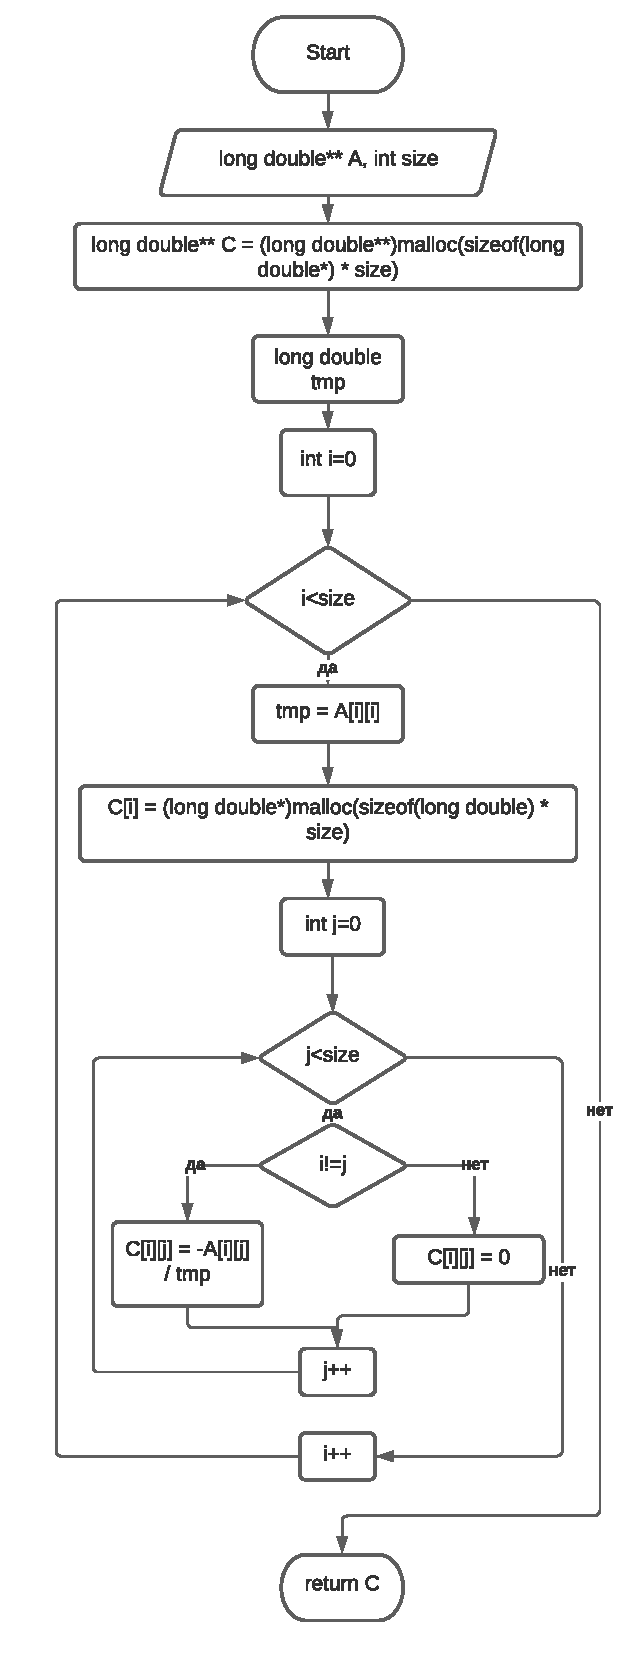
\includegraphics[scale=0.7]{block3.png}

double* OneVector(int size)

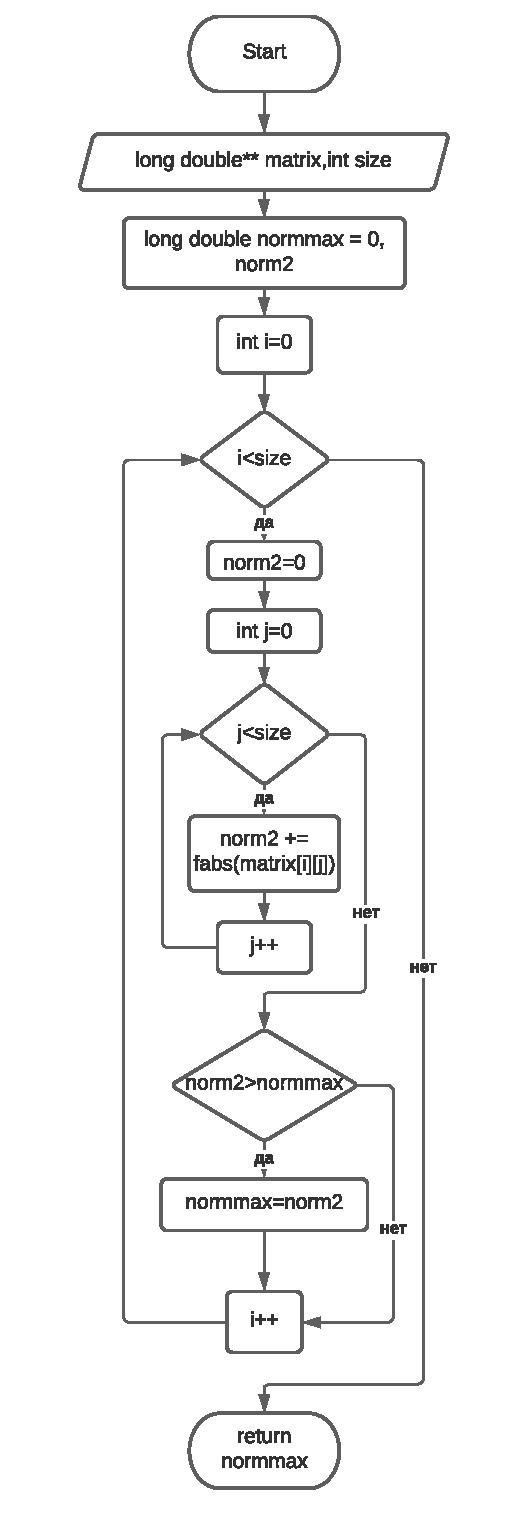
\includegraphics[scale=0.6]{block4.png}

double* MultVectorByNumber(double* vector, double number, int size)

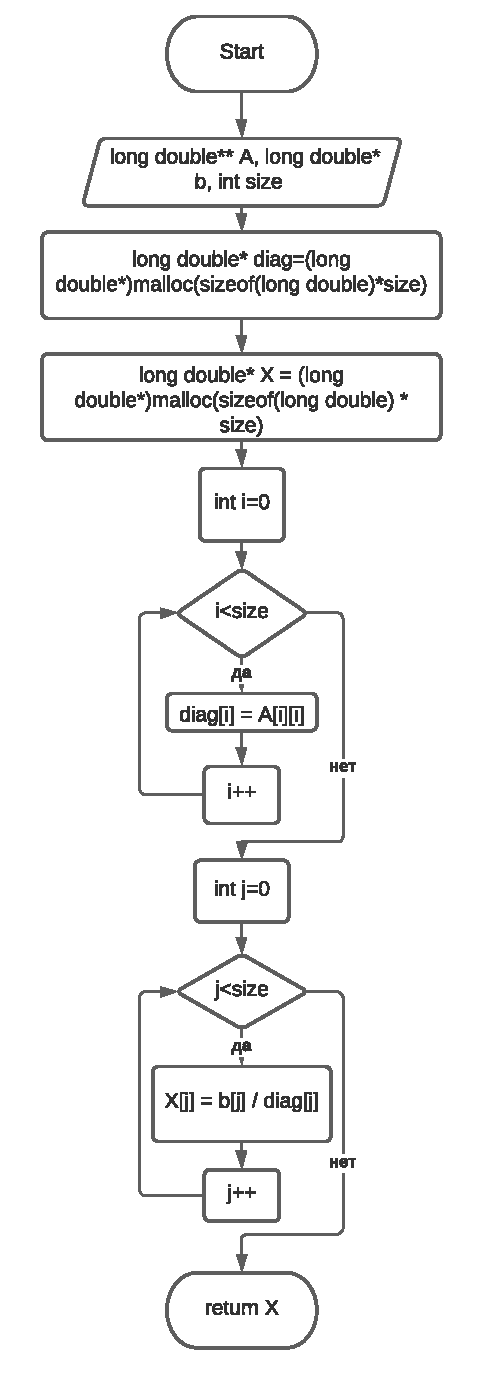
\includegraphics[scale=0.5]{block5.png}

double* SubstractionVector(double* X, double* Y, int size)

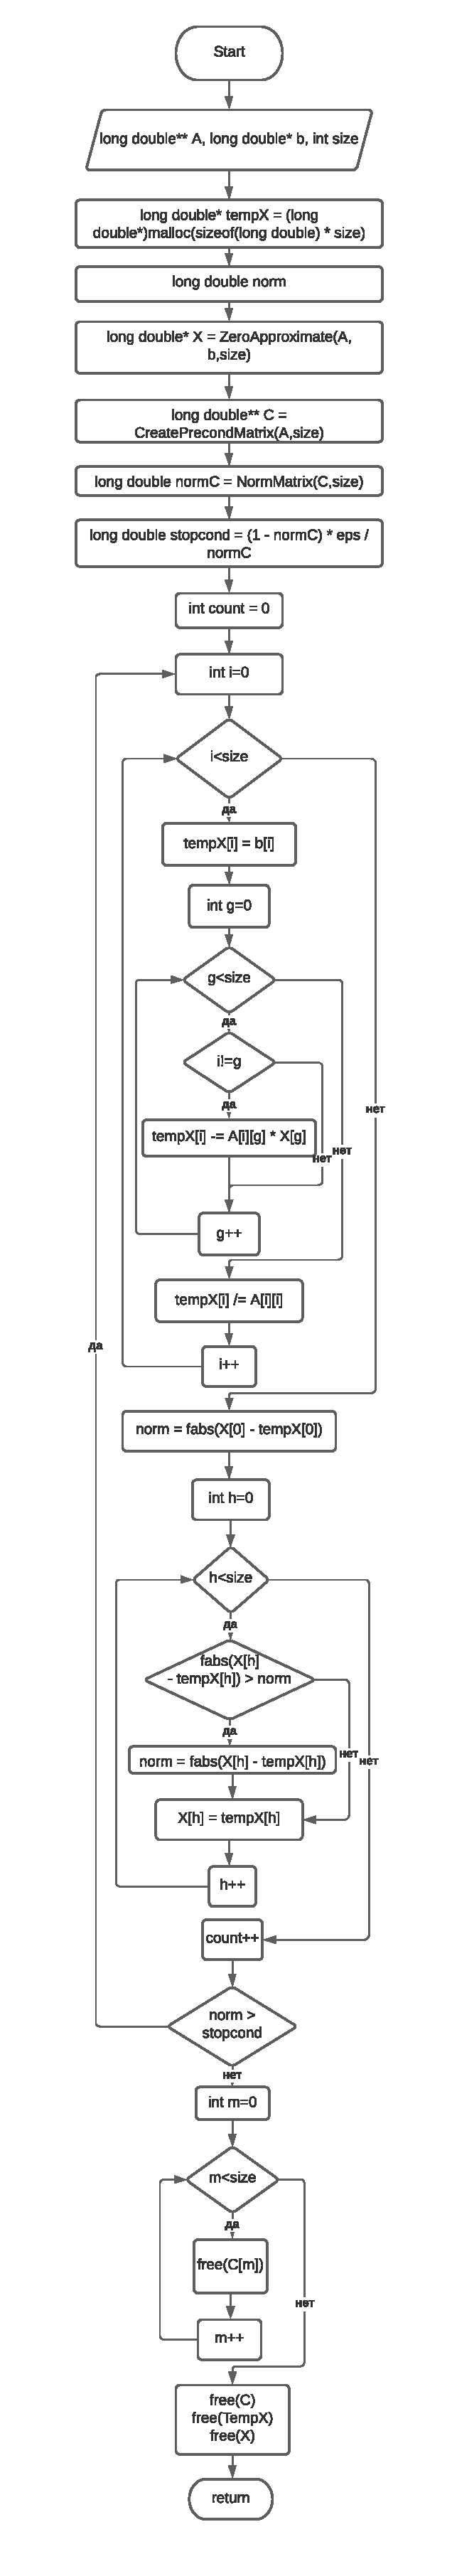
\includegraphics[scale=0.6]{block6.png}

void EqColumn(double* A, double* B, int size)

\includegraphics[scale=0.6]{block7.png}

double Norm2(double* vector, int size)

\includegraphics[scale=0.7]{block8.png}

double NormInf(double* vector, int size)

\includegraphics[scale=0.7]{block9.png}

double* PowerMethod1Eigen(double** matrix, int size)

\includegraphics[scale=0.6]{block10.pdf}

void PowerMethod2Eigen(double** matrix, double* eigen1vector, int size)

\includegraphics[scale=0.5]{block11.pdf}

\section{Численный анализ решения задачи}

\includegraphics[scale=0.75]{1.pdf}

На основе данного графика можно сделать вывод, что зависимость количества итераций от заданной точности является линейной в логарифмическом масштабе. Также можно заметить, что чем хуже отделимость, тем большее количество итераций потребуется для нахождения решения с заданной точностью.

\includegraphics[scale=0.75]{3.pdf}

Данный график подтверждает, что что чем хуже отделимость, тем большее количество итераций потребуется для нахождения решения с заданной точностью. 

\section{Краткие выводы}

Была решена задача нахождения нахождения второго собственного числа и соответствующего собственного вектора с помощью модификации степенного метода. 

Можно сделать вывод, что при использовании степенного метода для нахождения второго максимального по модулю СЧ лучше использовать при хорошей отделимости собственных чисел, иначе затраты на вычисления будут довольно большими.

\end{document}
